\documentclass{article}
\usepackage{amsmath}
\usepackage{listings}
\usepackage{tikz}
\usepackage{makeidx}
\usepackage{glossaries}
\makeindex
\makenoidxglossaries
\newglossaryentry{tex}{name={\TeX}, description={the typesetting system by Knuth}}
\newglossaryentry{satex}{name={SaTeX}, description={a checker that reads the document the way \TeX{} does}}
\lstset{basicstyle=\ttfamily\small, columns=fullflexible}
\title{Reading \TeX{} the Way \TeX{} Does}
\author{A.\ Student}
\date{November 2026}
\begin{document}
\begin{titlepage}
  \centering
  {\Large A thesis on static analysis\par}
  \vspace{2cm}
  {\huge\bfseries Reading \TeX{} the Way \TeX{} Does\par}
  \vspace{1.5cm}
  {\large A.\ Student\par}
  \vfill
  {\large November 2026\par}
\end{titlepage}
\tableofcontents
\listoffigures
\listoftables
\clearpage
\section[Background]{Background and Motivation}\label{sec:background}
Literate programming~\cite{knuth84} and the \TeX book~\cite{knuth86}
come first. Section~\ref{sec:background} says why, and
Sections~\ref{sec:listings} and~\ref{sec:pictures} show code and a picture.

\subsection{Listings}\label{sec:listings}
Inside \texttt{lstlisting} every character is read verbatim, so percent
signs and braces need no escapes:
\begin{lstlisting}[language=TeX]
\def\twice#1{#1#1} % braces { and } stay text
\twice{ab}
\end{lstlisting}
The same, inline: \lstinline|\section{x} 100% & $|.

\subsection{Pictures}\label{sec:pictures}
Figure~\ref{fig:flow} draws the pipeline.
\begin{figure}[ht]
  \centering
  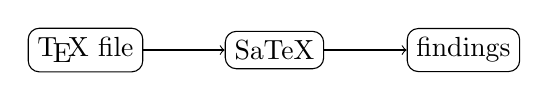
\begin{tikzpicture}[node distance=2.4cm, every node/.style={draw, rounded corners}]
    \node (tex) {\TeX{} file};
    \node (satex) [right of=tex] {SaTeX};
    \node (out) [right of=satex] {findings};
    \draw[->] (tex) -- (satex);
    \draw[->] (satex) -- (out);
  \end{tikzpicture}
  \caption[The pipeline]{From source to findings: \TeX{} reads, SaTeX checks}\label{fig:flow}
\end{figure}

\subsection{Cost}\label{sec:cost}
A run of $n$ lines with $k$ paths costs
\begin{equation}\label{eq:cost}
  T(n, k) = \sum_{i=1}^{n} c_i \cdot k_i \le c_{\max}\, n k ,
\end{equation}
so Equation~\eqref{eq:cost} bounds it by the longest line.
Joining two paths keeps both meanings:
\begin{align}
  m(p \sqcup q) &= m(p) \cup m(q), \label{eq:join}\\
  |m(p \sqcup q)| &\le |m(p)| + |m(q)| .
\end{align}
Table~\ref{tab:runs} lists measured runs.
\begin{table}[ht]
  \centering
  \begin{tabular}{lrr}
    Document & Lines & Seconds \\
    \hline
    article & 800 & 1.6 \\
    book & 3200 & 6.7 \\
  \end{tabular}
  \caption[Measured runs]{Measured runs of SaTeX on generated documents}\label{tab:runs}
\end{table}

\section{Terms}
\Gls{satex} reads the \gls{tex} source\index{source} and reports what it finds\index{finding}.
The macro\index{macro} definitions it sees are the ones \gls{tex} expands.
\printnoidxglossaries
\printindex
\bibliographystyle{plain}
\bibliography{refs}
% satex checks this on every path: the thesis stays short
%\satex@assert{\thepage < 9 and \value{section} >= 1}
\end{document}
